\subsection[Baum-Welch algorithm]{Learning from Observations:
  Baum-Welch algorithm}
\label{sec:bw}

\begin{frame}[t]
	\frametitle{Learning from observations - Reminder}
	\begin{block}{Model Estimation (Training) Problem}
    	Given some observed sequences, how do we adjust the \alert{parameters} of an HMM model that best tries 	
    	to explain the observations?
  	\end{block}
  	\pause
  	
  	\begin{block}{}
  		Adjust the model parameters $\lambda = (A, B, \Pi)$ to obtain $\max_{\lambda} P(O \vert \lambda)$
  	\end{block}
  	\pause
  	
  	\begin{block}{}
  		The observation sequence used to adjust the model parameters is called a \alert{training} sequence.\\
  		Training problem is crucial - allows to create best models for real phenomena.
  	\end{block}
\end{frame}


\begin{frame}[t]
	\frametitle{Learning from observations - Aspects of the approach}
	\pause
		
	\begin{block}{\alert{Problem}}
    	There is no known way to analytically solve for the model which maximizes the probability of the
    	observation sequence.
  	\end{block}
  	\pause
  	
  	\begin{block}{Solution}
  		We can choose $\lambda = (A, B, \Pi)$ such that $\max_{\lambda} P(O \vert \lambda)$ is 
  		\alert{locally maximized} using an \alert{iterative procedure} such as \emph{Baum-Welch}.\\
  		The method is an instance of the \emph{EM algoritm} \citep{dempster1977maximum} for HMMs.
  	\end{block}
  	
\end{frame}

\begin{frame}[t]
	\frametitle{Baum-Welch algorithm (I)}
	\pause
	We first define some auxiliary variables:
	
	\begin{block}{}    
    	$\xi_{t,i,j} = \xi_t(i,j) = P(q_t=s_i,q_{t+1}=s_j \vert O, \lambda)$\\
    	The probability of being in state $s_i$ at time $t$ and in state $s_j$ at time $t+1$, given
    	the model and the observation sequence.
	\end{block}
	\pause
	
	\begin{block}{}    
    	$ \gamma_{t,i} = \gamma_t(i) = P(q_t = s_i \vert O, \lambda)$\\
    	The probability of being in state $s_i$ at time $t$, given the model and the observation sequence.
	\end{block}
	\vspace*{1em}
	\pause
	
	From the definitions it follows that:\\
	$ \gamma_t(i) = \displaystyle\sum_{j=1}^{N}\xi_t(i,j)$
  	
\end{frame}

\begin{frame}[t]
	\frametitle{Baum-Welch algorithm (II)}
	\begin{columns}[T]
	
	\column{0.42\textwidth}
	\begin{figure}
  		\centering
		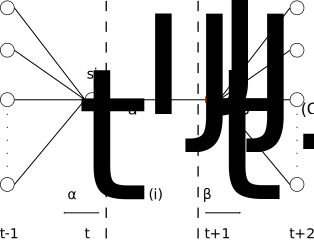
\includegraphics[height=0.40\textheight]{graphics/baum-welch/baum-welch-alg.pdf}
		\caption{\tiny{Sequence of operations required for the computation of the joint event that the system 
		is in state $S_i$ at time $t$ and state $S_j$ at time $t+1$} \citep{rabiner1989tutorial}}
		\label{fig:baum-welch-alg}
  	\end{figure}	
	
	\column{0.58\textwidth}
		\begin{equation*}		
		\alpha_{t,i}=P(o_1,o_2,\ldots,o_t, q_t = S_i \vert \lambda)
		\end{equation*}
		
		\begin{equation*}
		\beta_{t,i}=P(o_{t+1} o_{t+2} \cdots o_{T} \vert q_t = S_i, \lambda)
		\end{equation*}
		\footnotesize
		
		\begin{equation*}
			\begin{split}
		      \xi_t(i,j) & = \frac{\alpha_{t,i}\cdot a_{i,j} \cdot
		        b_j(o_{t+1}) \cdot \beta_{t+1,j}}
		      {P(O \vert \lambda)} \\
		      & = \frac{\alpha_{t,i}\cdot a_{i,j} \cdot b_j(o_{t+1}) \cdot
		        \beta_{t+1,j}}{
		        \displaystyle\sum_{k=1}^{N}\displaystyle\sum_{l=1}^{N}
		        \alpha_{t,k}\cdot a_{k,l} \cdot b_l(o_{t+1}) \cdot
		        \beta_{t+1,l}}
		    \end{split}
		\end{equation*}	
		\normalsize
	\end{columns}
	
\end{frame}

\begin{frame}
	\frametitle{Baum-Welch algorithm (III)}
	How do these auxiliary variables help?
	\vspace*{1em}
	
	\begin{block}{}
	$\displaystyle\sum_{t=1}^{T-1}\gamma_t(i)$ = expected number of transitions from $S_i$
	\end{block}
	\vspace*{1em}
	\begin{block}{}
	$\displaystyle\sum_{t=1}^{T-1}\xi_t(i,j)$ = expected number of transitions from $S_i$ to $S_j$
	\end{block}
	
\end{frame}

\begin{frame}[t]
	\frametitle{Baum-Welch algorithm (IV)}
	\footnotesize
	\begin{equation*}
	\bar{\pi_i} = \mbox{ expected no. of times in state } S_i \mbox{ at time } (t=1) = \gamma_t(i)
	\end{equation*}
	\pause	
	
	\begin{equation*}
	\begin{split}
	\bar{a_{i,j}} & = \frac{\mbox{expected no. of transitions from } S_i \mbox{ to } S_j}
							{\mbox{expcted no. of transition from } S_i} \\
				  & = \frac{\displaystyle\sum_{t=1}^{T-1}\xi_t(i,j)}
				   			{\displaystyle\sum_{t=1}^{T-1}\gamma_t(i)}	
	\end{split}
	\end{equation*}
	\pause	
	
	\begin{equation*}
	\begin{split}
	\bar{b_{j,k}}  & = \frac{\mbox{expected no. of times in } S_j \mbox{ observing symbol } v_k}
							{\mbox{expcted no. of times in } S_j} \\
				   & = \frac{\displaystyle\sum_{t=1, O_t = v_k}^{T}\gamma_t(j)}
				   			{\displaystyle\sum_{t=1}^{T}\gamma_t(j)}	
	\end{split}
	\end{equation*}	
	\normalsize	
\end{frame}

\begin{frame}[fragile, t]
	\frametitle{Baum-Welch algorithm (V)}
	The routine for the general case:
	\vspace*{1em}
    %     \lstset{columns=fullflexible, 
    %     		basicstyle=\footnotesize, 
    %     		numbers=left, 
    %     		stepnumber=1, 
    %     		numbersep=5pt,
    %     		title=Baum-Welch Iterative Update,
    %     		frame=single,
    %     		xleftmargin=1em,
    %     		captionpos=b}	

    %     \begin{lstlisting}[mathescape]
    % Initialize uniform $\pi_i$ for $1 \le i \le N$
    % Initialize random (stochastic) $a_{i,j}$
    % Initialize uniform $b_{j,k}$ for $1 \le k \le M$
	
    % Repeat until convergence
    %     E step:
    %         compute auxiliary variables $\xi_t(i,j)$ and $\gamma_t(i)$ 
    %         using current $\pi_i$, $a_{i,j}$ and $b_{j,k}$
        
    %     M step:
    %         compute updated parameter models $\bar{\pi_i}$, $\bar{a_{i,j}}$, $\bar{b_{j,k}}$
    %     \end{lstlisting}

\end{frame}

\begin{frame}
	\frametitle{Baum-Welch - Let's write some code}
	\centering
	LET'S WRITE SOME CODE :-)
\end{frame}